\documentclass[12pt]{article}
\usepackage[danish]{babel}
\usepackage{amsfonts, amssymb, mathtools, amsthm, amsmath}
\usepackage{graphicx, pgfplots}
\usepackage{url}
\usepackage[dvipsnames]{xcolor}
\usepackage{sagetex}
\usepackage{lastpage}

%loaded last
\usepackage[hidelinks]{hyperref}

\usepackage{siunitx}
  \sisetup{exponent-product = \cdot,
    output-decimal-marker = {,}}

%Giles Castelles incfig
\usepackage{import}
\usepackage{xifthen}
\usepackage{pdfpages}
\usepackage{transparent}

\newcommand{\incfig}[2][1]{%
  \def\svgwidth{#1\columnwidth}
  \import{../figures/}{#2.pdf_tex}
}

\setlength{\parindent}{0in}
\setlength{\oddsidemargin}{0in}
\setlength{\textwidth}{6.5in}
\setlength{\textheight}{8.8in}
\setlength{\topmargin}{0in}
\setlength{\headheight}{18pt}

\usepackage{fancyhdr}
\pagestyle{fancy}

\fancyhead{}
\fancyfoot{}
\fancyfoot[R]{\thepage}
\fancyhead[C]{\leftmark}

\pgfplotsset{compat=newest}

\pgfplotsset{every axis/.append style={
  axis x line=middle,    % put the x axis in the middle
  axis y line=middle,    % put the y axis in the middle
  axis line style={<->,color=black}, % arrows on the axis
}}

\usepackage{thmtools}
\usepackage{tcolorbox}
  \tcbuselibrary{skins, breakable}
  \tcbset{
    space to upper=1em,
    space to lower=1em,
  }

\theoremstyle{definition}

\newtcolorbox[auto counter]{definition}[1][]{%
  breakable,
  colframe=ForestGreen,  %frame color
  colback=ForestGreen!5, %background color
  colbacktitle=ForestGreen!25, %background color for title
  coltitle=ForestGreen!70!black,  %title color
  fonttitle=\bfseries\sffamily, %title font
  left=1em,              %space on left side in box,
  enhanced,              %more options
  frame hidden,          %hide frame
  borderline west={2pt}{0pt}{ForestGreen},  %display left line
  title=Definition \thetcbcounter: #1,
}

\newtcolorbox{greenline}{%
  breakable,
  colframe=ForestGreen,  %frame color
  colback=white,          %remove background color
  left=1em,              %space on left side in box
  enhanced,              %more options
  frame hidden,          %hide frame
  borderline west={2pt}{0pt}{ForestGreen},  %display left line
}

\newtcolorbox[auto counter, number within=section]{eks}[1][]{%
  brekable,
  colframe=NavyBlue,  %frame color
  colback=NavyBlue!5, %background color
  colbacktitle=NavyBlue!25,    %background color for title
  coltitle=NavyBlue!70!black,  %title color
  fonttitle=\bfseries\sffamily, %title font
  left=1em,            %space on left side in box,
  enhanced,            %more options
  frame hidden,        %hide frame
  borderline west={2pt}{0pt}{NavyBlue},  %display left line
  title=Eksempel \thetcbcounter: #1
}

\newtcolorbox{blueline}{%
  breakable,
  colframe=NavyBlue,     %frame color
  colback=white,         %remove background
  left=1em,              %space on left side in box,
  enhanced,              %more options
  frame hidden,          %hide frame
  borderline west={2pt}{0pt}{NavyBlue},  %display left line
}

\newtcolorbox{teo}[1][]{%
  breakable,
  colframe=RawSienna,  %frame color
  colback=RawSienna!5, %background color
  colbacktitle=RawSienna!25,    %background color for title
  coltitle=RawSienna!70!black,  %title color
  fonttitle=\bfseries\sffamily, %title font
  left=1em,              %space on left side in box,
  enhanced,              %more options
  frame hidden,          %hide frame
  borderline west={2pt}{0pt}{RawSienna},  %display left line
  title=Teori: #1,
}

\newtcolorbox[auto counter, number within=section]{sæt}[1][]{%
  breakable,
  colframe=RawSienna,  %frame color
  colback=RawSienna!5, %background color
  colbacktitle=RawSienna!25,    %background color for title
  coltitle=RawSienna!70!black,  %title color
  fonttitle=\bfseries\sffamily, %title font
  left=1em,              %space on left side in box,
  enhanced,              %more options
  frame hidden,          %hide frame
  borderline west={2pt}{0pt}{RawSienna},  %display left line
  title=Sætning \thetcbcounter: #1,
  before lower={\textbf{Bevis:}\par\vspace{0.5em}},
  colbacklower=RawSienna!25,
}

\newtcolorbox{redline}{%
  breakable,
  colframe=RawSienna,  %frame color
  colback=white,       %Remove background color
  left=1em,            %space on left side in box,
  enhanced,            %more options
  frame hidden,        %hide frame
  borderline west={2pt}{0pt}{RawSienna},  %display left line
}

\newtcolorbox{for}[1][]{%
  breakable,
  colframe=NavyBlue,  %frame color
  colback=NavyBlue!5, %background color
  colbacktitle=NavyBlue!25,    %background color for title
  coltitle=NavyBlue!70!black,  %title color
  fonttitle=\bfseries\sffamily, %title font
  left=1em,              %space on left side in box,
  enhanced,              %more options
  frame hidden,          %hide frame
  borderline west={2pt}{0pt}{NavyBlue},  %display left line
  title=Forklaring #1,
}

\newtcolorbox{bem}{%
  breakable,
  colframe=NavyBlue,  %frame color
  colback=NavyBlue!5, %background color
  colbacktitle=NavyBlue!25,    %background color for title
  coltitle=NavyBlue!70!black,  %title color
  fonttitle=\bfseries\sffamily, %title font
  left=1em,              %space on left side in box,
  enhanced,              %more options
  frame hidden,          %hide frame
  borderline west={2pt}{0pt}{NavyBlue},  %display left line
  title=Bemærkning:,
}

\makeatother
\def\@lecture{}%
\newcommand{\lecture}[3]{
  \ifthenelse{\isempty{#3}}{%
    \def\@lecture{Lecture #1}%
  }{%
    \def\@lecture{Lecture #1: #3}%
  }%
  \subsection*{\makebox[\textwidth][l]{\@lecture \hfill \normalfont\small\textsf{#2}}}
}

\makeatletter

\newcommand{\opgave}[1]{%
 \def\@opgave{#1}%
 \subsection*{Opgave #1}
}

\makeatother

%Format lim the same way in intext and in display
\let\svlim\lim\def\lim{\svlim\limits}

% horizontal rule
\newcommand\hr{
\noindent\rule[0.5ex]{\linewidth}{0.5pt}
}

\title{Opgaver til forelæsning uge 21}
\author{Noah Rahbek Bigum Hansen}
\date{20. November 2024}

\begin{document}

\maketitle

\section*{Opg. 11.1}
A \qty{0,120}{kg}, \qty{50,0}{cm}-long uniform bar has a small \qty{0,055}{kg}  mass glued to its left end and a small \qty{0,110}{kg}  mass glued to the other end. The two small masses can each be treated as point masses. You want to balance this system horizontally on a fulcrum placed just under its center of gravity. How far from the left end should the fulcrum be placed?
\bigbreak
Vi bruger formlen for massemidtpunkt fra en række masser i 1 dimension som
\[ 
x_c = \frac{\qty{0,055}{kg} \cdot 0 + \qty{0,120}{kg} \cdot \frac{\qty{50,0}{cm}}{2} + \qty{0,110}{kg} \cdot \qty{50,0}{cm}}{\qty{0,120}{kg} + \qty{0,055}{kg} + \qty{0,110}{kg}} = \qty{29,8}{cm} 
.\]



\section*{Opg. 11.2}
\begin{figure} [ht]
  \centering
  \caption{}
  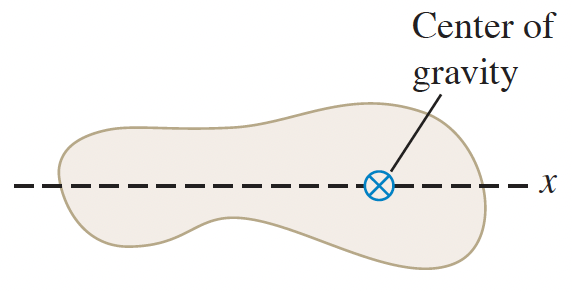
\includegraphics[width=0.35\linewidth]{../figures/E11_2.png}
  \label{fig:E11_2}
\end{figure}

The center of gravity of a \qty{5,00}{kg} irregular object is shown in \textbf{\autoref{fig:E11_2}}. You need to move the center of gravity \qty{2,20}{cm}  to the left by gluing on a \qty{1,50}{kg}  mass, which will then be considered as part of the object. Where should the center of gravity of this additional mass be located?
\begin{figure}[ht]
  \centering
  \incfig[0.35]{F21_11_2}
  \caption{Fritlegemediagram for situationen}
  \label{fig:F21_11_2}
\end{figure}
\bigbreak
Vi har at
\begin{align*}
  \Delta x = x_0 - \qty{2,20}{cm} &= \frac{mx_1 + Mx_0}{m + M} \\
  x_0(m + M) - \qty{2,20}{cm} (m + M) &= mx_1 + Mx_0 \\
  mx_1 &= x_0(m + M) - \qty{2,20}{cm} (m + M) - Mx_0 \\
  mx_1 &= m(x_0 - \qty{2,20}{cm}) - \qty{2,20}{cm} \cdot M  \\
  x_1 &= x_0 - \qty{2,20}{cm} - \qty{2,20}{cm} \frac{M}{m} \\
  x_1 &= \Delta x - \qty{2,20}{cm} \frac{M}{m}  \\
  x_1 &= \Delta x - \frac{\qty{2,20}{cm} \cdot \qty{5,00}{kg}}{\qty{1,50}{kg}}  \\
  x_1 &= \Delta x - \qty{7,333}{cm}  \\
  x_1 &= x_0 - \qty{9,533}{cm}
.\end{align*}



\section*{Opg. 11.19}
\begin{figure} [ht]
  \centering
  \caption{}
  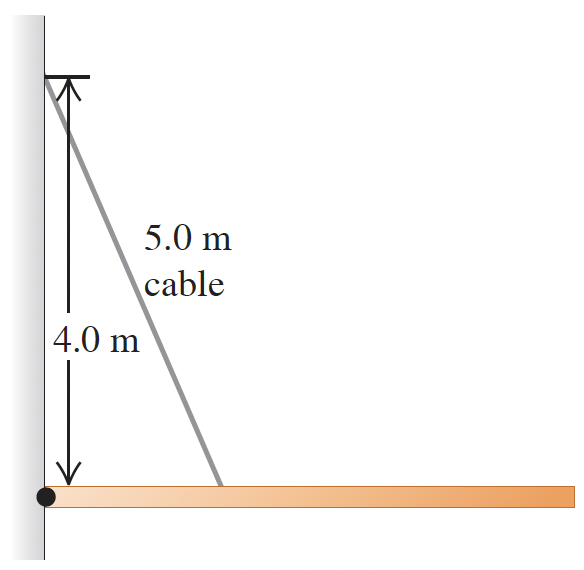
\includegraphics[width=0.3\linewidth]{../figures/E11_19.png}
  \label{fig:E11_19}
\end{figure}

A \qty{9,00}{m}-long uniform beam is hinged to a vertical wall and held horizontally by a \qty{5,00}{m}-long cable attached to the wall \qty{4,00}{m} above the hinge (\textbf{\autoref{fig:E11_19}}). The metal of this cable has a test strength of \qty{1,00}{kN}, which means that it will break if the tension in it exceeds that amount.


\subsection*{(a)}
Draw a free-body diagram of the beam.
\bigbreak
\begin{figure}[ht]
  \centering
  \incfig[0.8]{F21_11_19}
  \caption{Fritlegemediagram for situationen.}
  \label{fig:F21_11_19}
\end{figure}

Se \textbf{\autoref{fig:F21_11_19}}.

\subsection*{(b)}
What is the heaviest beam that the cable can support in this configuration?
\bigbreak
Kablet knækker ved $T = \qty{1,00}{kN}$. Vi skal altså finde størrelsen på $F_g$, der tilsvarer en spænding i kablet på $T = \qty{1,00}{kN}$. Idet der skal være statisk ligevægt har vi at
\[ 
\sum \tau_A = 0
.\]
Og dermed har vi at
\begin{align*}
  0 &= T_y \cdot \underbrace{\sqrt{(\qty{5,0}{m})^2 - (\qty{4,0}{m})^2}}_{\qty{3,0}{m}} - F_g \cdot \frac{\qty{9}{m}}{2} \\
  T_y &= F_g \cdot \frac{\qty{4,5}{m}}{\qty{3,0}{m}} \\
  T &=  F_g \cdot \frac{\qty{4,5}{m}}{\qty{3,0}{m} \cdot \sin(\underbrace{\theta}_{\tan^{-1} \left( \frac{4}{3} \right)})} \\
  T &= \num{1,875} F_g \\
  F_g &= \frac{\qty{1,00}{kN}}{\num{1,875}} = \qty{0.533}{kN} 
.\end{align*}


\subsection*{(c)}
Find the horizontal and vertical components of the force the hinge exerts on the beam. Is the vertical component upward or downward?
\bigbreak
Vi har, igen, statisk ligevægt og det gælder derfor at
\[ 
\sum F_x = 0
.\]
Vi har derfor
\begin{align*}
  0 &= T_x - A_x \\
  A_x &= T_x \\
  &= T \cos(\theta)  \\
  &= \qty{1,0}{kN} \cdot \frac{3}{5} = \qty{600}{N} 
.\end{align*}

Og vi kan gøre det samme for y-retningen som
\begin{align*}
  0 &= T_y + A_y - F_g \\
  A_y &= \qty{0.533}{kN} - \frac{4}{5}T \\
  &= \qty{0,533}{kN} - \qty{0,800}{kN} = \qty{-0.267}{kN}
.\end{align*}


\section*{Opg. 11.47}
\begin{figure} [ht]
  \centering
  \caption{}
  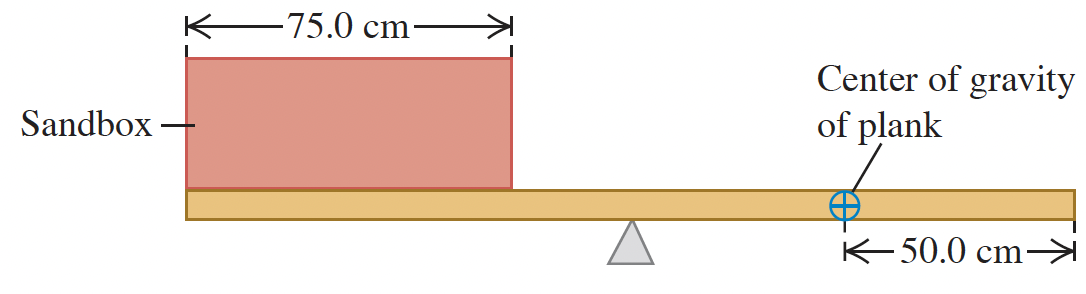
\includegraphics[width=0.5\linewidth]{../figures/P11_47.png}
  \label{fig:P11_47}
\end{figure}

A box of negligible mass rests at the left end of a \qty{2,00}{m}, \qty{25,0}{kg} plank (\textbf{\autoref{fig:P11_47}}). The width of the box is \qty{75,0}{cm}, and sand is to be distributed uniformly throughout it. The center of gravity of the nonuniform plank is \qty{50,0}{cm} from the right end. What mass of sand should be put into the box so that the plank balances horizontally on a fulcrum placed just below its midpoint?
\bigbreak
Vi sætter $x_{cm} = \qty{0}{cm}$ til at være netop ved det ønskede balancepunkt. Startmassemidtpunktet er da $x_p = \frac{\qty{200}{cm}}{2} - \qty{50,0}{cm} = \qty{50,0}{cm}$. Massemidtpunktet for kassen er placeret ved $x_k = - \frac{\qty{200}{cm}}{2} + \frac{\qty{75,0}{cm}}{2} = \qty{-62,5}{cm}$. Vi kan da opstille formlen for massemidtpunktet
\begin{align*}
  x_{cm} = \qty{0}{cm} &= \frac{x_p \cdot m_p + x_k \cdot m_k}{m_p + m_k} \\
  &= x_p \cdot m_p + x_k \cdot m_k \\
  m_k &= \frac{-x_p \cdot m_p}{x_k} \\
  &= \frac{- \qty{50}{cm} \cdot \qty{25,0}{kg}}{-\qty{62,5}{cm}} \\
  &= \qty{20,0}{kg}  
.\end{align*}


\section*{Opg. 11.49}
\begin{figure} [ht]
  \centering
  \caption{}
  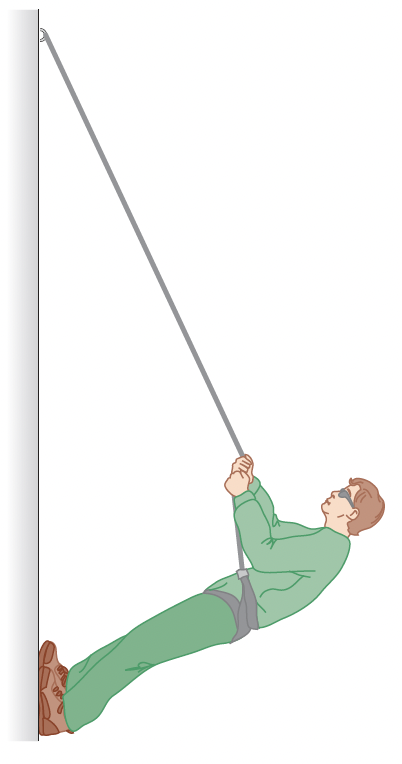
\includegraphics[width=0.15\linewidth]{../figures/P11_49.png}
  \label{fig:P11_49}
\end{figure}

\textbf{Mountain Climbing.} Mountaineers often use a rope to lower themselves down the face of a cliff (this is called \textit{rappelling}). They do this with their body nearly horizontal and their feet pushing against the cliff (\textbf{\autoref{fig:P11_49}}). Suppose that an \qty{82,0}{kg} climber, who is \qty{1,90}{m} tall and has a center of gravity \qty{1,1}{m} from his feet, rappels down a vertical cliff with his body raised \ang{35,0} above the horizontal. He holds the rope \qty{1,40}{m} from his feet, and it makes a \ang{25,0} angle with the cliff face.

\subsection*{(a)}
What tension does his rope need to support?
\begin{figure}[ht]
  \centering
  \incfig[0.3]{F21_11_49}
  \caption{Fritlegemediagram for situationen.}
  \label{fig:F21_11_49}
\end{figure}

Vi har statik og derfor må det gælde at
\[ 
\sum \tau = 0
.\]
Og dermed får vi at
\begin{align*}
  0 &= -F_g \cdot \cos \left( \ang{35}  \right) \cdot l_{cm} + T \cdot \cos \left( \ang{10}  \right) \cdot l_{tot}  \\
  T &= F_g \frac{\cos \left( \ang{35}  \right) \cdot l_{cm}}{\cos \left( \ang{10} \right) \cdot l_{tot}} \\
  T &= \qty{0.786}{m} \cdot F_g = \qty{525.191}{kN} 
.\end{align*}



\subsection*{(b)}
Find the horizontal and vertical components of the force that the cliff face exerts on the climber’s feet.
\bigbreak
Grundet samme overvejelser om statik som i opg. 11.19 har vi at
\[ 
\sum F_x = 0
.\]
Og vi får da, at
\begin{align*}
  0 &= N - T \cdot \sin \left( \ang{25}  \right) \\
  N &= \qty{221,955}{kN} 
.\end{align*}

Og det samme kan gøres i y-retningen som
\begin{align*}
  0 &= T \cdot \cos \left( \ang{25} \right) - F_g + F_{\mu} \\
  F_{\mu} &= F_g - T \cdot \cos \left( \ang{25} \right) \\
  &= \qty{82,0}{kg} \cdot \qty{9,8}{\frac{m}{s^2}} - \qty{525,191}{kN} \cdot \cos (\ang{25}) = \qty{327,788}{kN} 
.\end{align*}

\subsection*{(c)}
What minimum coefficient of static friction is needed to prevent the climber’s feet from slipping on the cliff face if he has one foot at a time against the cliff?
\bigbreak
Gnidningskoefficienten findes ved brug af formlen for gnidningskraft som
\begin{align*}
  F_\mu &= \mu \cdot N \\
  \mu &= \frac{F_{\mu}}{N} \\
  &= \frac{\qty{327,788}{kN}}{\qty{221,955}{kN}} = \num{1,4769}  \\
.\end{align*}



\section*{Opg. 11.71}
\begin{figure} [ht]
  \centering
  \caption{}
  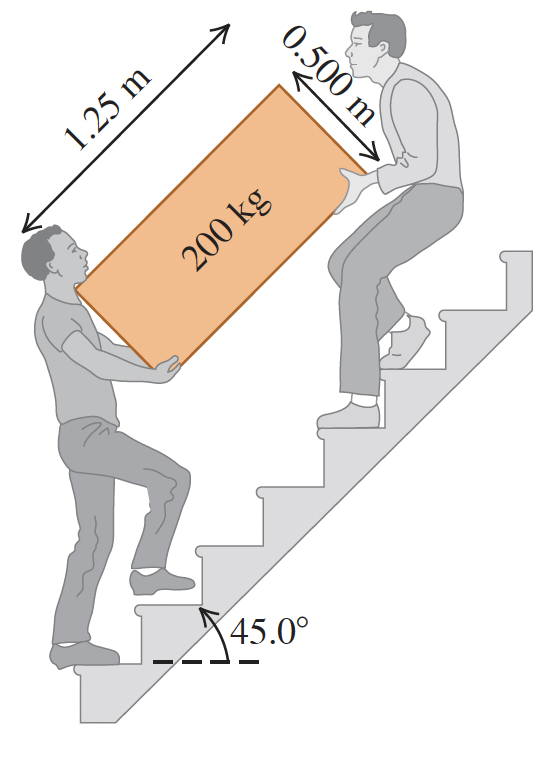
\includegraphics[width=0.15\linewidth]{../figures/P11_71.png}
  \label{fig:P11_71}
\end{figure}


Two friends are carrying a \qty{200}{kg} crate up a flight of stairs. The crate is \qty{1,25}{m} long and \qty{0,500}{m} high, and its center of gravity is at its center. The stairs make a \ang{45,0} angle with respect to the floor. The crate also is carried at a \ang{45,0} angle, so that its bottom side is parallel to the slope of the stairs (\textbf{\autoref{fig:P11_71}}). If the force each person applies is vertical, what is the magnitude of each of these forces? Is it better to be the person above or below on the stairs?

\begin{figure}[ht]
  \centering
  \incfig[0.8]{F21_11_71}
  \caption{Fritlegemediagram}
  \label{fig:F21_11_71}
\end{figure}

\bigbreak
Vi sætter 0-punktet til at være netop det hjørne som den nederste person holder i. Vi får da at tyngdekraftet laver et moment $\tau_1$ med udgangspunkt i tyngdekraften fra kassens massemidtpunkt og at den anden person laver et moment $\tau_2$ med udgangspunkt i den kraft han løfter kassen med. Se evt. \textbf{\autoref{fig:F21_11_71}}.

Idet der er statik har vi, at
\[ 
  \sum F_y = F_1 + F_2 - F_g = 0
\]
og
\[ 
  \sum \tau = F_2 \cdot \qty{1,25}{m} \cdot \cos(\ang{45}) - \frac{\qty{1,25}{m}}{2} \cdot F_g \cdot \cos(\ang{45}) + \frac{\qty{0,500}{m}}{2} \cdot F_g \cdot \sin(\ang{45}) = 0
.\]
Eftersom $\cos(\ang{45}) = \sin(\ang{45})$ har vi at
\begin{align*}
  F_2 \cdot \qty{1,25}{m} \cdot \cos(\ang{45}) &= \frac{\qty{1,25}{m}}{2}\cdot F_g \cdot \cos(\ang{45}) - \frac{\qty{0,500}{m}}{2}\cdot F_g \cdot \sin(\ang{45}) \\
  F_2 \cdot \qty{1,25}{m} &= \frac{\qty{1,25}{m} - \qty{0,500}{m}}{2}\cdot F_g \\
  F_2 &= \frac{\qty{1,25}{m} - \qty{0,500}{m}}{2 \cdot \qty{1,25}{m}} \cdot F_g \\
  &= \num{0,3} F_g \\
  &= \num{0,3} \cdot \qty{200}{kg} \cdot \qty{9,80}{\frac{m}{s^2}} = \qty{588}{N} 
.\end{align*}
Altså er kraften som den øverste person skal udøve $F_2 = \qty{588}{N}$. Dette kan nu indsættes i udtrykket for $\sum F_y$ for at finde kraften som den nederste person skal udøve $F_1$ som
\[ 
F_1 = F_g - F_2 = F_g - \num{0,3}F_g = \num{0,7} \cdot \qty{200}{kg} \cdot \qty{9,80}{\frac{m}{s^2}} = \qty{1372}{N} 
.\]
Altså er det bedst at stå i toppen.


\end{document}
